%        File: ivarhs.tex
%     Created: Thu Mar 05 07:00 PM 2015 C
% Last Change: Thu Mar 05 07:00 PM 2015 C
%
\documentclass[a4paper]{article}

% Language and encoding
\usepackage[utf8]{inputenc} 

% Mathematical typesetting
\usepackage[]{amsmath} 
\usepackage[]{amsthm}
\usepackage[]{amssymb} 

% Graphics and figures
\usepackage[]{graphicx}

% Codelistings
\usepackage[]{minted} 

% Custom sectioning commands
\newtheorem{prb}{Problem}
\theoremstyle{definition}
\newtheorem{sol}{Solution}
\newcommand{\horrule}[1]{\rule{\linewidth}{#1}}

% Title
\title{
  \textsc{University of Oslo} \\
  \textsc{Assignment 1} \\
  \textsc{STK1100}
}
\author{Ivar Haugaløkken Stangeby}
\date{\today}

\begin{document}
\maketitle

\begin{prb}
  In a game of roulette the roulette wheel is subdivided into 37 numbered
  fields. The fields are alternating red and black with the field numbered 0 as
  the only green field.  Assuming a player bets 100\$ on a group consisting of
  $k$ fields, and the ball stops at one of them, the player wins
  $100\cdot(36/k)$\$. If, on the other hand, the ball stops at any of the other
  fields, the player lose their bet of 100\$.  Assuming we are looking at a
  player that are involved in $20$ games, and every time the player bets 100\$
  at 18 fields.
\end{prb}

\begin{sol}
\item\paragraph{a)} 
Since we are looking at a scenario where there for each spin of the wheel are
two different outcomes, the player either wins or loses. The probability $p$ of
winning is constant across all $n = 20$ games. Therefore, $X$, being the number
of wins in 20 games, is binomially distributed.

We want to examine the expected value of $X$, that is - what is the expected
number of wins given 20 games and with a probability $p$?
\begin{equation}
  \label{eq:ex}
  \mathbb{E}\left( X \right) = \sum_{x = 1}^{n = 20} x\cdot p(x) = \sum_{x =
  1}^{n = 20} x \cdot {n \choose x} \cdot p^{x} \cdot \left( 1-p \right)^{n-1}
  = np.
\end{equation}
The simplification of \eqref{eq:ex} to $np$ can be shown using Newton's binomial theorem.
Evaluating this for $n = 20$ and $p = \frac{18}{37}$ we get:
\begin{equation}
  \notag
  \mathbb{E}\left( X \right) = \mu_X = np = 20\cdot \frac{18}{37} \approx 9.73.
\end{equation}

In order to find the standard deviation of $X$, $SD(X)$, we must first find the variance $\mathbb{V}(X)$.
\begin{align*}
  \mathbb{V}(X) &= \mathbb{E}\left(\left(X-\mu_X\right)^{2}\right) = \mathbb{E}\left( X^{2} \right) - \mu_X^{2} = \mathbb{E}\left( X^{2} \right) - \mu_{X} \\
  &= \sum_{x=1}^{n=20} x^{2} p(x) - \mu_X^{2} \approx 99.66 - 94.66 = 4.99 = \sigma_{X}^{2}.
\end{align*}
Based on this, we can find the standard deviation $SD(X) = \sigma_{X}$.
\begin{equation}
  \notag
  \sigma_{X} = \sqrt{\sigma_{X}^{2}} \approx \sqrt{4.99} = 2.23.
\end{equation}

\paragraph{b)}
Letting $Y$ be the collected net gain in the 20 games we see that we can write $Y$ in terms of
the number of won games $X$: 
\begin{align*}
  \notag
  Y &= 100 \cdot \left( \frac{36}{18} - 1 \right) \cdot X - 100\cdot\left( n - X \right)\\
    &= 200 \cdot (X - 10).
\end{align*}
To find the expected value of $Y$ we observe that $Y(X)$ is a linear function, therefore we can write:
\begin{equation}
  \notag
  \mathbb{E}\left( Y \right) = \mathbb{E}\left( 200\left( X-10 \right) \right) = 200\mathbb{E}\left( X \right) - 2000.
\end{equation}
Evaluating this, we find:
\begin{equation}
  \notag
  \mu_{Y} = 200\mu_{X} - 2000 \approx -54.
\end{equation}
Now, for the variance of $Y$. This can easily be found by using the fact that $\mathbb{V}(aX + b) = a^2\mathbb{V}(X)$.
Thus:
\begin{equation}
  \notag
  \mathbb{V}(Y) = \sigma_{Y}^{2} = 200^2 \mathbb{V}\left( X \right) \approx 200^{2} \cdot 4.99 = 199600.
\end{equation}
Based on this, the standard deviation $\sigma_{Y}$ is equal to
\begin{equation}
  \notag
  \sigma_{Y} = \sqrt{199600} \approx 446.77
\end{equation}

\paragraph{c)}
We now want to investigate what the probability of winning a certain number of money.
We do this by looking at the cumulative distribution of $Y$ in terms of $X$.
First off, we want to find the probability that the player wins at least $1000$.
We want to write this probability in terms of the random variable $X$.

\begin{align*}
  P(Y \geq 1000) &= P(200X - 2000 \geq 1000) = P(X \geq 15) \\
  &= 1 - P(X \leq 14) = 1 - F(14) =  1 - \sum_{x=0}^{14} p(x)\\
  &\approx 0.015 
\end{align*}

Now, we want to find the probability that the player loses more than $1000$.
That is, 
\begin{equation}
  \notag
  P(Y \leq -1000)
\end{equation}
Again, we write $Y$ in terms of $X$ and use the cumulative distribution of $X$.

\begin{align*}
  P(Y \leq -1000) &= P(200X - 2000 \leq -1000) = P(X \leq 5) \\
  &= F(5) = \sum_{x=0}^{5}p(x) \approx  0.027
\end{align*}

\paragraph{d)}

We're now reducing the number of fields the player bets on from 18 to 6. We
therefore have to rewrite our $Y$ random variable.  We also have to update our
probability $p = \frac{6}{37}$.  In this situation, we have
\begin{equation}
  \notag
  Y = 100\cdot\left( \frac{36}{6} - 1\right)X - 100\left( 20-X \right) = 600X - 2000.
\end{equation}

Using the same method as above, we get 
\begin{align*}
  \label{eq:}
  P(Y \geq 1000) = P(X \geq 5) = 1 - P(X \leq 4) = 0.214, \\
  P(Y \leq -1000) = P(X \leq \frac{5}{3}) = P(X \leq 1) = 0.000032.
\end{align*}

\paragraph{e)}
We're now looking at a player repeatedly bets 100\$ on a single field until he
wins once, then he stops playing. Letting $Z$ denote the number of times he
plays. This gives us $p = \frac{1}{37}$ and $Y$ in terms of $Z$:
\begin{equation}
  \notag
  Y = -100(Z - 1) + 3500 = -100Z + 3600
\end{equation}
The probability distribution for $Z$ is a special case of the negative binomial
distribution.  Since the player keeps playing until he has won once, we're
looking at the probability of $Z - 1$ losses followed by a win.  The
probabilities for playing $x$ times is given as follows: (Since there is only
one way of distributing $Z-1$ losses in $Z$ games, we can disregard the
binomial coefficient.) This is what we call the geometric probability
distribution.
\begin{equation}
  \notag
  p(x) = p\cdot(1-p)^{x-1}, \quad x \in \mathbb{N}.
\end{equation}

\paragraph{f)}

We're now examining the probability that the player wins at least 1000, and the
probability that he loses more than a 1000.

\begin{align*}
  P(Y \geq 1000) &= P(-100Z + 3600 \geq 1000) = P(Z \leq 26) \\
  &= F(26) \approx 0.51 \\
  P(Y \leq -1000) &= P(-100Z + 3000 \leq -1000) \\
  &= 1 - P(Z \geq 46) \approx 0.28
\end{align*}
\end{sol}

\begin{prb}
  Letting the stocastic variable $X$ denote the womans remaining years in whole
  years. That is, the lifespan in whole years subtracted 30. We want to
  determine the point probability $p(x) = P(X = x)$ for this stocastic
  variable.
\end{prb}

\begin{sol}
\item\paragraph{a)}
  Let $q_x$ denote the probability that a $x$ year old person dies within one year.
  We want to show that the cumulative distribution function $F(X)$ is then $F(X) = 1 - S(X)$,
  where
  \begin{equation}
    \notag 
    S(X) = P(X > x) = \prod\limits_{y=0}^{x} \left( 1 - q_{30+y} \right).
  \end{equation}
  The probability that a person dies within $x$ years is given by 1 minus the
  probability said person lives longer than $x$ years.  The probability that a
  person lives longer than $x$ years is the probability that the person lives 1
  year longer, multiplied by the probability that the person lives 2 years
  longer, and so on and so forth all the way to to $x$ years.  Therefore, it is
  easily deduced that $F(X) = 1 - S(X)$.

\paragraph{b)}
We want to figure out what the probability of having exactly $x$ years remaining.
This has to be the probability of dying within $x$ years, minus the probability of dying within $x-1$ years.
Therefore,
\begin{equation}
  \notag
  p(x) = F(x) - F(x-1).
\end{equation}
\end{sol}

\paragraph{c)}
Below is a graph of the point probability of dying within $x$ years past the age of 30.
\begin{figure}[h]
  \centering
  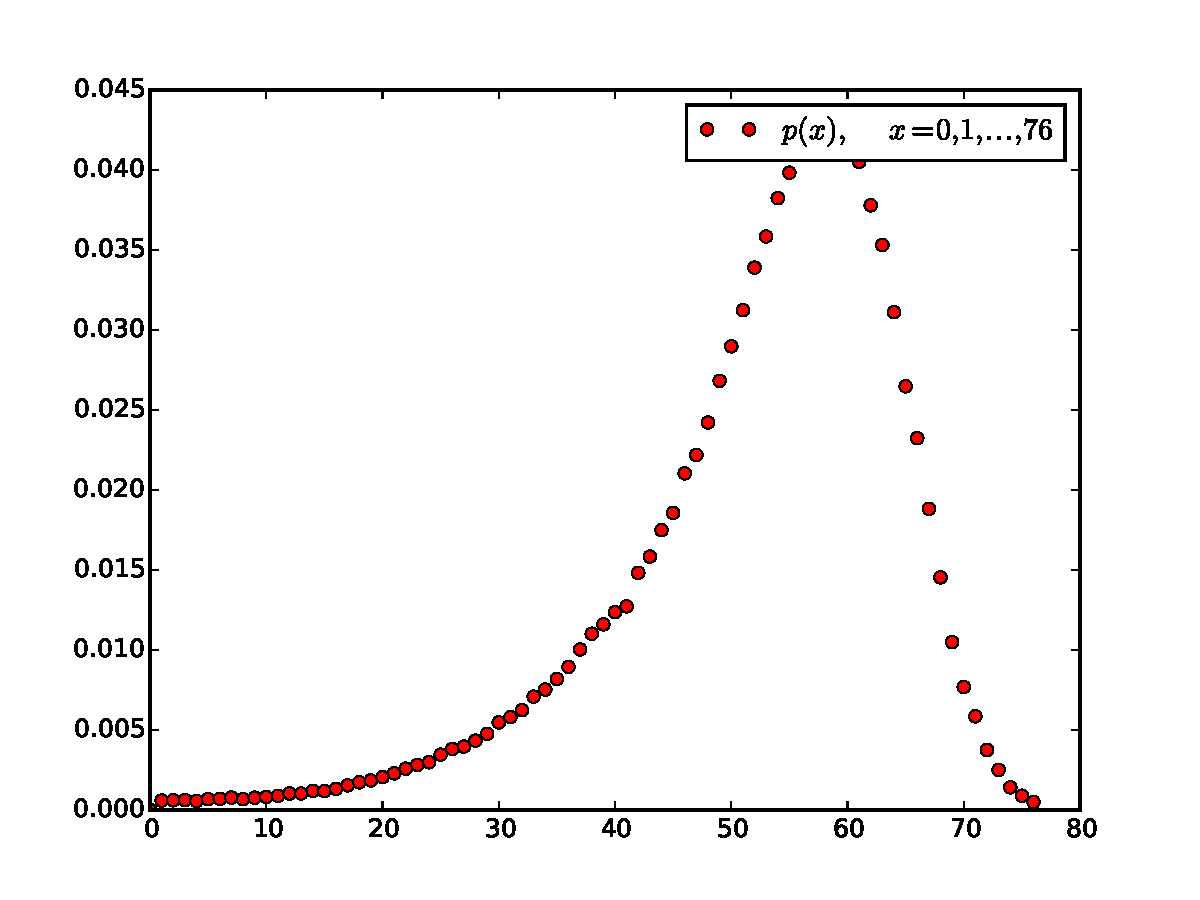
\includegraphics[width=0.7\linewidth]{./src/point_probability.pdf}
  \caption{Point probability $p(x)$ versus $x$}
  \end{figure}
\paragraph{d)}
Let $h\left( X \right)$ denote the payment of compensation. Since we're working
with an interest of $3\%$ the value of $B$ payed in $k$ years is equal to
$B/1.03^k$.  We can therefore define $h(X)$ as the piecewise function
\begin{equation}
  \notag
  h\left( X \right) = \left\{\begin{array}{lr}
    \frac{1000000}{1.03^X} & : X \leq 35 \\
    0 & : X \geq 35
    \end{array}
  \right..
\end{equation}

\paragraph{e)}

The expected value of $h(X)$ is given given by the sum over the product of the
probability of $X = x$ and the payment of compensation for $X = x$ from $x=0$
to $x = 76$. In other words, 
\begin{equation}
  \notag
  \mathbb{E}\left[ h(X) \right] = \sum_{x=0}^{76}h(x)p(x).
\end{equation}
Since $h(X)$ is defined to be zero for $X \geq 35$, the weighted probability is
zero for any $X$'s greater than 35. Therefore we can disregard these
terms.  Written out, this becomes:
\begin{equation}
  \label{eq:expct}
  \mathbb{E}\left[ h(X) \right] = \sum_{x=0}^{34} \frac{1000000p(x)}{1.03^x} = 1000000\sum_{x=0}^{34}\frac{p(x)}{1.03^x}.
\end{equation}

\paragraph{f)}
Using \eqref{eq:expct} and the point probabilities from \textbf{c} we can calculate
the expected present value of payment of compensation.
Running my \textsc{Python}-script, we get the value:
\begin{equation}
  \notag
  \mathbb{E}\left[ h(X) \right] = 38579.72.
\end{equation}

\paragraph{g)}
The woman pays an annual premium of $K$ from the age of $30$ and all the way to
the age of $64$, if she is alive. This means, that we want to sum the annual
premium from $k = 0$ all the way up to the minimum of $X$ and $34$. And then
multiply it with $K$.  Therefore we can write the total premium payment as
\begin{equation}
  \notag
  K \cdot \left( \frac{1 - (1/1.03)^{\min\left( X, 34 \right)+1}}{1 - 1/1.03} \right).
\end{equation}

\paragraph{h)}
The expected present value of the womans total premium payments must
neccessarily be given as $K \cdot \mathbb{E}\left[ g(X) \right]$ since $K$ is
constant and $\mathbb{E}\left[ g(X) \right]$ is the expected number of annual
payments.

From the definition, we have
%TODO Finish this
\begin{align*}
  \label{eq:}
  \mathbb{E}\left[ g(X) \right] &= \sum_{x=0}^{76}g(x)p(x)
\end{align*}

\paragraph{i)}
Using the formula from \textbf{h} and the point probability from \textbf{c}, we
calculate the expected value of $g(X)$.  Running my \textsc{Python}-script I
get the value:
\begin{equation}
  \notag
  \mathbb{E}\left[ g(X) \right] \approx 21.76
\end{equation}
\paragraph{h)}

The annual premium $K$ is given by:
\begin{equation}
  \notag
  K \cdot \mathbb{E}\left[ g(X) \right] = \mathbb{E}\left[ h(X) \right].
\end{equation}
Solving this for $K$, we get:
\begin{equation}
  \notag
  K \approx \frac{38579.72}{21.76} = 1772.96.
\end{equation}

\section*{Code}
\inputminted[samepage=true]{python}{./src/point_probability.py}
\end{document}
